\documentclass[10pt,twocolumn]{article}

% ------------------ PAQUETES ------------------
\usepackage[spanish]{babel}
\usepackage[utf8]{inputenc}
\usepackage[T1]{fontenc}
\usepackage{geometry}
\usepackage{graphicx}
\usepackage{amsmath, amssymb}
\usepackage{siunitx}
\usepackage{authblk}
\usepackage{abstract}
\usepackage{caption}
\usepackage{titlesec}
\usepackage{multicol}
\usepackage{hyperref}
\usepackage{currfile}
\usepackage{float}

\geometry{margin=1.8cm}

% ------------------ FORMATO DE SECCIONES ------------------
\titleformat{\section}{\large\bfseries}{\thesection}{1em}{}
\titleformat{\subsection}{\normalsize\bfseries}{\thesubsection}{1em}{}

% ------------------ TÍTULO ------------------
\title{\textbf{Aproximación manual a la fotometría de apertura}\\Trabajo sobre el cúmulo abierto Messier 41}


% ------------------ AUTORES ------------------
\author[1]{Bruno Abello Laurent}

\affil[1]{Universidad de Los Andes, Departamento de Física, Colombia}

% Correos (puedes modificar)
\renewcommand\Authands{, }
\date{}

\begin{document}

\twocolumn[
\maketitle
\begin{center}
\small
\textit{Correo institucional:} \href{mailto:{b.abello@uniandes.edu.co}}{b.abello@uniandes.edu.co} \\
\textit{Repositorio de GitHub: } \href{https://github.com/Brunelleschk1/Personal-projects/tree/main/Proyectos\%20de\%20Astronom\%C3\%ADa/Laboratorio\%202}{Repositorio del laboratorio}
\end{center}

\begin{abstract}
\noindent
Aquí va el resumen del informe. Debe describir brevemente el objetivo, metodología, resultados principales y conclusiones.
\end{abstract}

\noindent\textbf{Palabras clave:} palabra1, palabra2, palabra3
\vspace{0.5cm}
]

% ------------------ CONTENIDO ------------------

\section{Introducción}

``En palabras simples, nos quedamos cortos cuando se trata de determinar la pertenencia de un centroide a un cúmulo. 
Por lo tanto, a lo largo de la próxima semana se trabajará en los métodos que permiten una mejor determinación de pertenencia, 
pero esta vez con datos de GAIA, debido a la imposibilidad de definir movimientos propios de cuerpos celestes con una sola imagen.''

Con estas palabras se terminó el trabajo de la semana pasada. Efectivamente, nuestro método de estudio del cúmulo Messier 41 es bastante anticuado y, 
como observamos, muy bueno para detectar estrellas pero muy malo para decidir cuáles son efectivamente parte del cúmulo. 

El día de hoy, por ende, decidimos avanzar en nuestros conocimientos y nuestros métodos. Ahora, con dos mil estrellas cuyos datos se descargaron de GAIA dr3,
vamos a interesarnos a un nuevo tipo de diagrama, el VPD(Vector Point Diagram). Este nos permite visualizar un cluster de una manera mucho más clara,
y esto se debe a la particularidad que los astrofísicos detectaron sobre los cúmulos después de la segunda guerra mundial, y es que los movimientos propios
de sus estrellas son supremamente similares entre sí. Claro, esto es normal ya que todas esas estrellas nacieron al tiempo y están muy juntas, en la 
escala astronómica. 

Mediante el estudio de los movimientos propios de las estrellas, junto con un ajuste de optimización de parámetros gaussianos, es posible determinar
con una alta precisión qué estrellas pertenecen al cúmulo y qué estrellas pertenecen al campo. Este documento es un informe sobre los problemas que 
presentó la implementación del método, sus limitaciones y sus poderosas fortalezas. 


\subsection{Objetivos}

Los objetivos que tenemos, en términos simples, son los siguientes:
\begin{itemize}
    \item Acercarnos a funciones computacionales cada vez más cercanas a lo que se utiliza en la astrofísica moderna.
    \item Empezar a familiarizarnos con las particularidades de los algoritmos de aprendizaje automático e iterativo.
    \item Aprender a leer un Vector Point Diagram y a interpretarlo.
    \item Aprender a interpretar los resultados probabilísticos del método de optimización de parámetros.
    \item Aprender a determinar qué es un problema en la programación y qué es un problema de los datos utiizados.
\end{itemize}


\section{Procedimiento}

Similarmente al laboratorio anterior, el procedimiento fue, al igual que el método, iterativo. A través de la prueba y error, 
se fue implementando una función de optimización de parámetros cada vez más ajustada a lo que se solía utilizar en la
astrofísica. Esto se logró mediante la descarga de datos de GAIA en el área próxima a Messier 41 en un CSV, formato
de fácil lectura en python. Para los valores iniciales que toma la función se utilizaron unos valores encontrados por
otro estudiante del curso, por lo cual se esperaban valores similares a estos. 

Una vez estos valores obtenidos, se imprimen y se realizan varias gráficas: un nuevo VPD con el cúmulo resaltado, 
un histograma de probabilidades de pertenencia al cúmulo según cada estrella, y un CMD con las estrellas del 
cúmulo resaltadas. 

El proceso se puede describir como iterativo, ya que, como era de esperarse, estuvo lleno de inconvenientes y
de revisiones.

\section{Problemas presentados y soluciones aplicadas}

\begin{enumerate}
  \item Por la cantidad de dudas que generan los parámetros ajustados, el código se hizo en tres documentos separados. 
  El primero fue bastante sencillo, con errores de normalización y de cálculos. El siguiente arregló muchas cosas, pero no la normalización, 
  y el último normalizó la gaussiana(por fin) y fue donde empezó a ser importante hablar de los demás problemas importantes.
  \item El método no convergió a los valores esperados para la dispersión del cluster(0.2633 esperado vs 0.1637 obtenido),
   mu x y y del campo(esperados -0.7410 y 0.6275 vs -0.5297 y 0.3883 obtenidos), sigma y del campo(7.3140 vs 6.6971) y n del campo(0.9455 vs 0.6798).
   \item Debido a esto, se empezaron a aplicar una serie de controles y de maneras de ver si el método computacional estaba fallando. 
   \begin{enumerate}
    \item No tenía un problema con el orden de interpretación y asimilación de los parámetros de las gaussianas, la función recibía todo en orden.
    \item La normalización de la función no jugó un papel importante en devolver los parámetros a lo esperado, es más disminuyó el nf en dos puntos.
    \item La coloración por probabilidad de pertenencia del VPD no mostró estrellas alejadas del "cúmulo" con probabilidades remotamente altas de pertenecer(Fig.~\ref{VPDViejoZOOM}). 
    \item Los conteos con threshold de 0.9 o más de probabilidad de pertenecer muestran una cantidad de estrellas supremamente cercana a la encontrada por nf y por demás métodos.
    \item El histograma de probabilidades, si bien en escala logarítmica no parece tan drástico, es supremamente binario en escala normal en cuanto a pertenecer o no (Fig.~\ref{ProbPertViejo}).
    \item los percentiles más altos(>75) de la distribución de probabilidad dieron todos superiores a 0.9, confirmando la binariedad de la probabilidad de pertenencia.
    \item 529 estrellas tienen una probabilidad de 99 porciento de pertenecer al cúmulo.
    \item La distancia en unidades de sigma entre estas 529 estrellas no supera los 2.7 sigmas, por lo que no se tratan de un montón de outliers que la optimización no detectó (Fig.~\ref{DistSigmViejo}).
    \item La densidad de estrellas en el cúmulo decrece con la distancia en minutos de arco, lo que es esperable.
    \item La distribución de estrellas pertenecientes en un diagrama de declinación recta contra declinación disminuye conforme nos vamos alejando del centro, como se espera. (Fig.~\ref{RADecViejo}) 
   \end{enumerate}
\end{enumerate}

Con esto dicho, se considera que la mejor manera de presentar lo que siguió a continuación es en la sección de análisis de resultados. 

\subsection{Figuras de los problemas}

\begin{figure}[H]
    \centering
    
\includegraphics[width=0.8\linewidth]{../CosasErrNorm/VPD_Pmayor0_zoomcluster.png}
    \caption{VPD del primer set de datos utilizado. Se puede observar una gran densidad de estrellas en el cúmulo, con muy poquitas por fuera 
    con probabilidades de pertenencia mucho más bajas}
    \label{VPDViejoZOOM}
\end{figure}

\begin{figure}[H]
    \centering
    
\includegraphics[width=0.8\linewidth]{../CosasErrNorm/ProbPertU.png}
    \caption{Gráfico de probabilidad de pertenencia en función de cada estrella. Se aprecia que la distribución es supremamente binaria. }
    \label{ProbPertViejo}
\end{figure}

\begin{figure}[H]
    \centering
    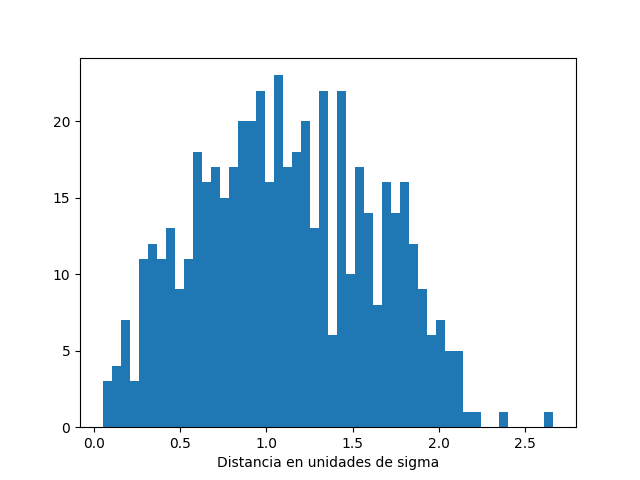
\includegraphics[width=0.8\linewidth]{../CosasErrNorm/Distancia_en_sigmas.png}
    \caption{Distancia, en sigmas de la distribución, entre las estrellas encontradas por la función de optimización de parámetros. 
    Una distancia tan baja supone que los elementos sí pertenecen todos al cúmulo, sin excepciones reales.}
    \label{DistSigmViejo}
\end{figure}

\begin{figure}[H]
    \centering
    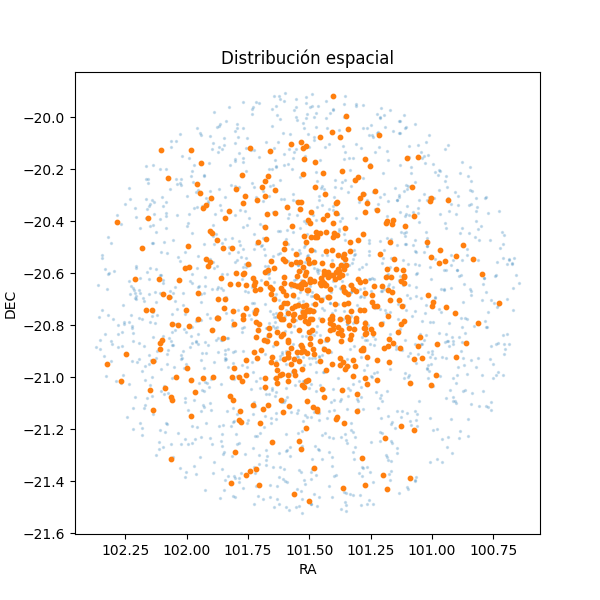
\includegraphics[width=0.8\linewidth]{../CosasErrNorm/Distribución_espacial_RA_Dec.png}
    \caption{Mapa de la ascención recta contra la declinación de cada elemento analizado. En anaranjado se muestran los pertenecientes 
    al cúmulo, mostrando que, efectivamente, la mayoría se encuentran en una zona de alta densidad hacia el centro de la agrupación. }
    \label{RADecViejo}
\end{figure}

Otros resultados mencionados incluyen: 

75, 90, 95, 99, 100 percentiles de Probabilidad

[0.99345065 0.9981174  0.99854258 0.99877663 0.99882815]

Estrellas con P>0.9: 599

Estrellas con P>0.99: 529

Tal y como los imprime el código: "Código con errores Normalizado.py", disponible en la ruta Laboratorio 2/Código con errores Normalizado.py 

\section{Resultados}

Evidentemente, el set de datos presentaba algún problema:  El cluster se ve perfectamente y está extrañamente bien definido, con unas probabilidades altísimas para muchas estrellas.
Después de tantas pruebas, la única respuesta lógica era que el set de datos tenía algo extraño. Gracias al archivo de datos de otro compañero, se hicieron las mismas pruebas, 
corriendo el mismo código, para el nuevo archivo. Estas pruebas están en la ruta Laboratorio 2/Lab 2 Otro csv.
El resultado fue flagrante: 5 porciento de pertenencia al cúmulo por parte de la población, valores de optimización tales y como
se esperaban, unas 100 estrellas en el cúmulo contra las más de 500 encontradas anteriormente, pocas estrellas con una probabilidad tan alta de pertenecer al cúmulo, 
pero una buena población por encima de 0.7. (Fig.~\ref{PertUNuevoLog}) Entonces, se aplicó un test directamente a los archivos .csv para determinar su correlación. 
Resultado, una sola estrella presente entre los dos archivos. Todo el análisis inicial, que duró varios días, se había hecho sobre una región del cielo que, 
sí, efectivamente, posee un cúmulo, pero que claramente no es Messier 41. Las semejanzas son, sin embargo, impresionantes, 
ya que ambos cúmulos se encuentran más o menos en la misma región de sus respectivos VPD, y algunos de sus datos de optimización son muy similares. 

Ya con el set de datos correcto, se puede empezar a hablar mejor de lo que encuentra el código. Para simplificar las cosas, y no tener que buscar manualmente en un VPD 
cada una de las estrellas coloreadas, se realizó un VPD que tome las estrellas con probabilidad superior a un threshold y las muestre. De esta manera, 
se obtiene un VPD de buena calidad que muestra correctamente el cluster y sus alrededores. (Fig.~\ref{VPDNuevoZOOM}). Se ven claramente las estrellas que pertenecen y las que pueden pertenecer, 
y el CMD ya presenta resultados en una región aceptable y esperada. (Fig.~\ref{CMDNuevo}). Un par de preguntas resultan de la distribución de probabilidades, ya que es cierto que no es
una distribución tan binaria como se espera.(Fig.~\ref{PertUNuevoLog}). Sin embargo, se obtiene en el VPD un resultado coherente y que parece un cúmulo bien definido. 

\begin{figure}[H]
    \centering
    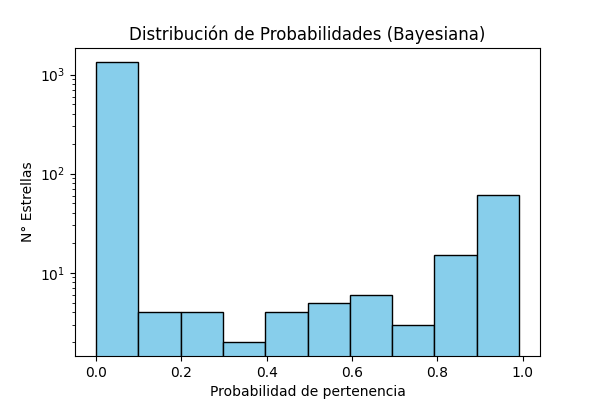
\includegraphics[width=0.8\linewidth]{../Lab2Otrocsv/CosasErrNorm/ProbPertU.png}
    \caption{Diagrama de probabilidad de pertenencia en función de cada estrella para el nuevo set de datos en escala logarítmica.
    Una comparación al histograma sin esta escala se encuentra en el anexo. \ref{PertUNuevo}}
    \label{PertUNuevoLog}
\end{figure}

\begin{figure}[H]
    \centering
    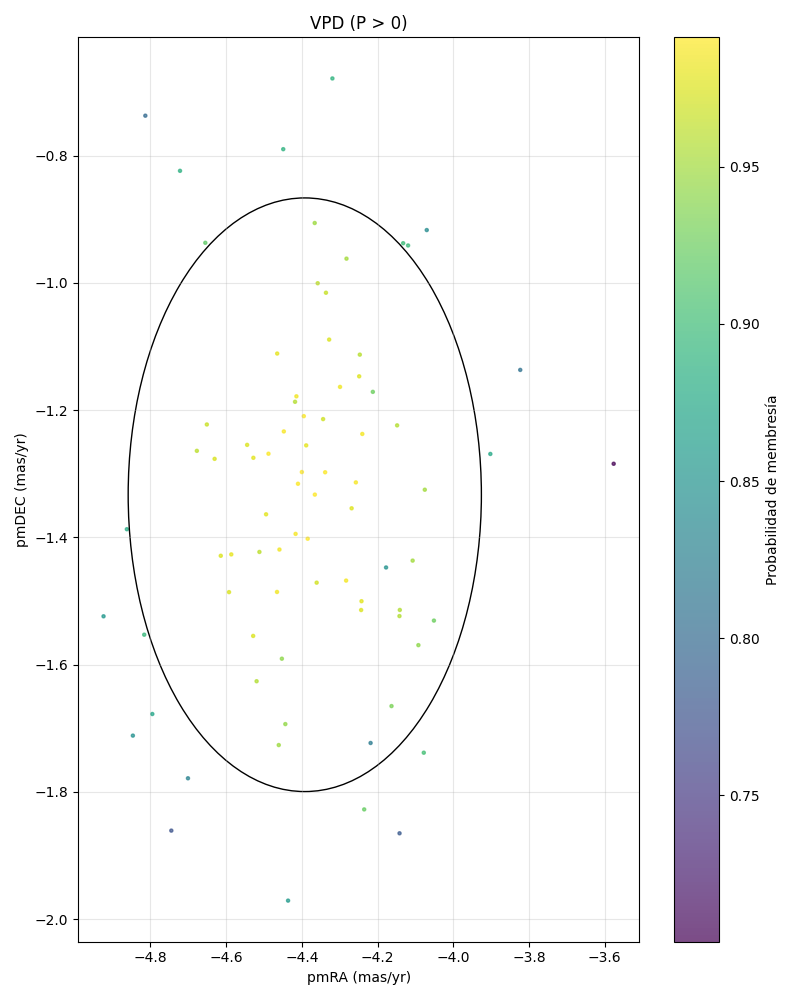
\includegraphics[width=0.8\linewidth]{../Lab2Otrocsv/CosasErrNorm/VPD_Pmayor0_zoomcluster.png}
    \caption{VPD de los miembros con P>0.7 de pertenecer al cúmulo. Se oberva una densidad mucho menor de estrellas que en (Fig.~\ref{VPDViejoZOOM}).
    Asimismo, se ve que ciertas estrellas dentro de la zona resaltada no tienen una probabilidad tan alta de pertenecer al cúmulo.}
    \label{VPDNuevoZOOM}
\end{figure}

\begin{figure}[H]
    \centering
    
\includegraphics[width=0.8\linewidth]{../Lab2Otrocsv/CosasErrNorm/CMDPintadoErr.png}
    \caption{CMD del nuevo set de datos. Se observa una población mayoritariamente en la parte inicial de la secuencia principal, tal y como se esperaba
    al iniciar este laboratorio. Comparado al CMD viejo, se nota que los resultados cuadran con lo esperado. (Fig.~\ref{CMDViejo}) }
    \label{CMDNuevo}
\end{figure}

\begin{figure}[H]
    \centering
    
\includegraphics[width=0.8\linewidth]{../Lab2Otrocsv/CosasErrNorm/RADEC.png}
    \caption{Diagrama de declinación contra ascención recta. Comparado a (Fig.~\ref{RADecViejo}), se observa una zona diagonal dibujada, 
    a comparación de la densidad central que se diluye hacia los bordes. Esto significa que nuestro cúmulo es ahora mucho más pequeño
    y menos definido. }
    \label{RADECNuevo}
\end{figure}

Otro problema notable es el gráfico de ascención recta contra declinación de este set de datos. (Fig.~\ref{RADECNuevo}). Lo que empezó como una manera de asegurarse de que el ''cúmulo''
de 500 estrellas era de verdad un cúmulo terminó siendo una herramienta útil para dudar del cúmulo M41. Se supone que, en este gráfico, los valores correspondientes
a las estrellas pertenecientes al cúmulo deberían estar en una región cercana, y cercana al centro del gráfico. Sin embargo, lo que presenta este caso es que no hay
tanta claridad en cuanto a dónde está el cúmulo en este mismo. Algunas estrellas están muy arriba, otras muy abajo, otras en el medio, casi como una diagonal 
ancha que atraviesa el diagrama de abajo a la izquierda a arriba a la derecha. También se realizó un estudio de la distancia en sigmas entre la población con 
más de 0.7 de probabilidad de pertenecer al cúmulo en cuanto a sus proper motions, y se encontraron un par de estrellas por encima de los 5 sigmas, lo que indica
que el cúmulo ya se está extendiendo un poco por encima de lo que se ve normalmente. (Fig.~\ref{SIGMANuevo}).

\begin{figure}[H]
    \centering
    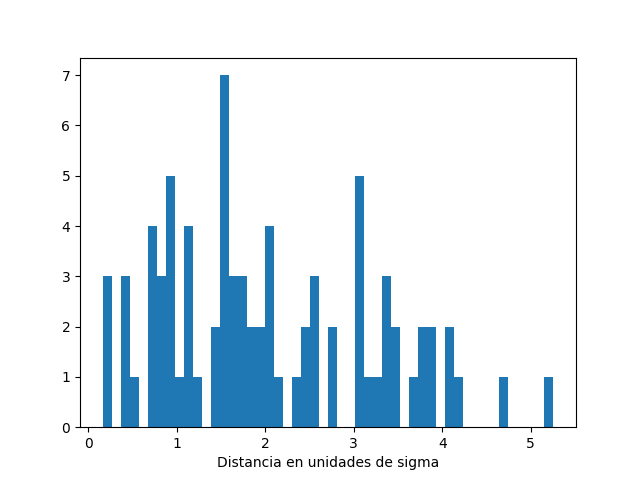
\includegraphics[width=0.8\linewidth]{../Lab2Otrocsv/CosasErrNorm/Sigmas.png}
    \caption{Histograma de la distancia en sigmas entre las estrellas con P>0.7 de pertenecer a M41. Se observan distancias más grandes que en el anterior, (Fig.~\ref{DistSigmViejo}) pero se siguen teniendo muchas 
    estrellas cercanas a lo esperado y solo unas cuantas por encima de los 5 sigmas, lo que significa que, a pesar de estar más diluido que el anterior, sigue siendo un cúmulo bien definido.}
    \label{SIGMANuevo}
\end{figure}

Por último, solamente 3 estrellas pertenecen con más de 99 porciento de confianza, y solo 79 con más del 70. Estos números son bastante contrariantes,
ya que se esperarían unos 100 miembros en el cluster\cite{wikipedia_messier41}. Sin embargo, el CMD muestra muchos miembros en la zona de enanas blancas,
antes de entrar a la secuencia principal, y pocos miembros en la misma, lo que es de esperarse en un estudio como este. 
Es decir, el resultado obtenido, si bien es poco satisfactorio, es lo que se esperaba obtener, y posiblemente los miembros de la secuencia principal
que no aparecen en nuestro CMD son precisamente los que faltan en nuestro conteo probabilístico. 

\section{Conclusiones}

Es, entonces, evidente que nuestro método se queda una vez más muy corto para poder determinar la pertenencia de una estrella a un cúmulo, como ya se ha dicho.
Por una parte, no se encuentran todas las estrellas que se esperaban. Esto no es de esperarse, ya que, normalmente, se descargó la región del cielo en la que
se sabe que está el cluster. Sin embargo, es el método que implementamos lo que más sorpresas da. Como se dijo, presenta problemas de definición de pertenencia, 
aunque muchos menos que el de hace una semana. Asimismo, presenta un bias en los miembros encontrados hacia la base de la secuencia principal, 
lo que conocemos como incorrecto ya que el cúmulo M41, bien estudiado, presenta miembros a lo largo de la secuencia principal. 

Gracias a solo dos semanas de implementación computacional, encontramos las razones por las cuales ningún método tradicional de computación resulta ser
suficiente para estudiar cúmulos galácticos. A partir de la próxima semana, por ende, optamos por iniciar nuestra investigación en el territorio 
del Machine Learning. Para permitirnos un estudio a profundidad, descargaremos un nuevo set de datos con muchísimos más datos. Nótese la robustez
de los métodos de Machine Learning, que podremos importar miles de datos y aún así encontrar nuestro cúmulo bien definido. Eso esperamos, al menos. 

\section*{Referencias}

\bibliographystyle{apalike}
\bibliography{refs}

\section*{Comentarios al margen}


\section*{Imágenes adicionales}

\begin{figure}[H]
    \centering
    
\includegraphics[width=0.8\linewidth]{../Lab2Otrocsv/CosasErrNorm/ProbPertUNoLog.png}
    \caption{Diagrama de probabilidad de pertenencia en función de cada estrella para el nuevo set de datos.
    Se observa a duras penas la diferencia entre la pertenencia más alta al cúmulo y las probabilidades inferiores. }
    \label{PertUNuevo}
\end{figure}

\begin{figure}[H]
    \centering
    
\includegraphics[width=0.8\linewidth]{../CosasErrNorm/CMDPintadoErr.png}
    \caption{CMD del primer set de datos estudiado. Se puede evidenciar una población perteneciene casi exclusivamente perteneciente a 
    La secuencia principal, algo que no es lo esperado cuando se trabaja con este método de optimización de parámetros.}
    \label{CMDViejo}
\end{figure}

\end{document}